\documentclass[11pt]{article}
\usepackage[T1]{fontenc}
\usepackage{lmodern}
\usepackage[a4paper,margin=28mm]{geometry}
\usepackage{amsmath,amssymb,amsthm}
\usepackage{booktabs}
\usepackage{graphicx}
\usepackage[colorlinks=true,linkcolor=blue,citecolor=blue,urlcolor=blue]{hyperref}
\usepackage{microtype}

\newtheorem{theorem}{Theorem}[section]
\newtheorem{lemma}[theorem]{Lemma}
\newtheorem{proposition}[theorem]{Proposition}
\newtheorem{corollary}[theorem]{Corollary}
\newcommand{\CC}{\mathbb C}
\newcommand{\rank}{\operatorname{rank}}
\newcommand{\arank}{\widetilde{\operatorname{rank}}}
\newcommand{\vd}{V_{\mathrm d}}
\newcommand{\ud}{U_{\mathrm d}}
\newcommand{\eps}{\varepsilon}
\newcommand{\degen}{\unrhd}
\newcommand{\cmm}[3]{\langle #1,#2,#3\rangle}
\DeclareMathOperator{\MM}{MM}

\title{Rectangular matrix multiplication from shared-leg entropy}
\author{Przemysław Uznański\thanks{This note was obtained with the assistance
of OpenAI Codex (GPT-6.1). The author has read and analyzed this note in full
and takes full responsibility for its contents.}\\[2pt]\small Pathway}
\date{October 7, 2026}

\begin{document}
\maketitle

\begin{abstract}
In this note, we extend the matrix-multiplication analysis of~\cite{openai-2026-matrix-nine-fourths} to
rectangular products and prove
\[
 \omega(1,k,1)\le
 \begin{cases}
 2,&0\le k\le \frac{1}{2},\\
 1+k+1/(4k),&k\ge \frac{1}{2}.
 \end{cases}
\]
In particular, $\omega(1,\frac{1}{2},1)=2$ and the dual exponent satisfies
$\alpha\ge \frac{1}{2}$. We use the shared-leg entropy inequality and
polynomial-multiplication degenerations of OpenAI, retaining two-leg
symmetry and the orientation of each sector. Logarithmic averaging
produces homogeneous auxiliary profiles. Their powered versions have
a common asymptotic slope, and bounding their intercepts gives the
spectral constraint $b\le 4a(1-a)$. This yields the rectangular curve
by tensor-spectrum duality. As an application, Zwick's algorithm
\cite{zwick-2002-bridging-sets} for all-pairs shortest paths in directed
unweighted graphs runs in $O_\eps(n^{2.5+\eps})$ time for every $\eps>0$.
\end{abstract}

\section{Introduction}\label{sec:statement}

Rectangular matrix multiplication is a basic ingredient in algorithms
for all-pairs problems, including shortest paths, lowest common ancestors,
and Hamming distance. Its exponents depend on the shape of the product;
an improvement for square matrices need not give a comparable
improvement for every rectangular shape.
OpenAI~\cite{openai-2026-matrix-nine-fourths} proved the square bound
$\omega\le9/4$ using a shared-leg entropy inequality and degenerations
of polynomial-multiplication tensors. We extend that analysis to
rectangular products by retaining the orientation information lost
under full leg symmetrization.

For fixed nonnegative real $u,v,w$, let $\omega(u,v,w)$ be the infimum
of the exponents $e$ for which, for every $\eps>0$, multiplying an
$\lceil n^u\rceil\times\lceil n^v\rceil$ matrix by a
$\lceil n^v\rceil\times\lceil n^w\rceil$ matrix uses
$O_{u,v,w,\eps}(n^{e+\eps})$ arithmetic operations over $\CC$.
Write $f(k)=\omega(1,k,1)$ and
$\alpha=\sup\{k\ge0:f(k)=2\}$.

\begin{theorem}\label{thm:curve}
For every fixed real $k\ge0$,
\begin{equation}\label{eq:curve}
 f(k)\le F(k):=
 \begin{cases}
 2,&0\le k\le \frac{1}{2},\\[2pt]
 1+k+\dfrac1{4k},&k\ge\frac{1}{2}.
 \end{cases}
\end{equation}
Consequently $f(k)=2$ for $0\le k\le\frac{1}{2}$, $\alpha\ge\frac{1}{2}$, and
$f(2)\le25/8$.
\end{theorem}

Applying the square bound to square blocks gives only
$f(k)\le2+k/4$ for $0\le k\le1$ and $f(k)\le k+5/4$ for $k\ge1$.
Theorem~\ref{thm:curve} instead gives exponent two for inner dimension
up to $n^{\frac{1}{2}}$, and an upper bound within $1/(4k)$ of the input-size
lower bound $1+k$ for $k\ge1$.

\begin{figure}[tbp]
 \centering
 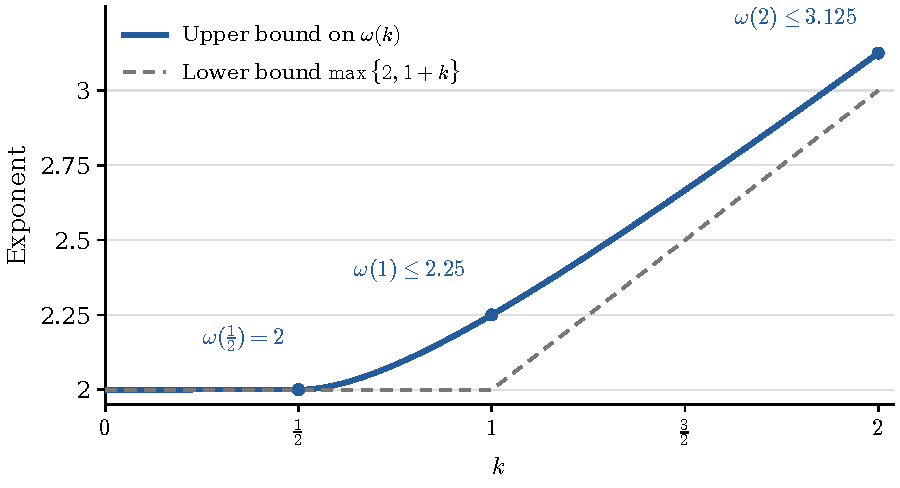
\includegraphics[width=0.86\linewidth]{figures/rectangular-exponent-curve.pdf}
 \caption{The upper bound $F(k)$ from Theorem~\ref{thm:curve} for
 $0\le k\le2$, together with the size lower bound
 $\max\{2,1+k\}$. The bounds coincide for
 $0\le k\le\frac{1}{2}$.}
 \label{fig:rectangular-curve}
\end{figure}

Our proof bounds the dot-product parameters of every tensor character.
After averaging over the interchange of two legs, these parameters
have the form $(a_0,a_0,b_0)$, and the rectangular objective is
$2a_0+kb_0$. We prove the parabolic constraint
$b_0\le4a_0(1-a_0)$. The main step is a logarithmic homogenization of
two oriented polynomial-multiplication profiles. Their coupled
tripling inequalities force a common asymptotic slope and control
the intercepts, producing the parameter constraint. Optimizing the
rectangular objective then proves the theorem.

\section{Tensor characters and polynomial multiplication}\label{sec:discrete}

We use the standard tensor-spectrum formulation. A character $\lambda$
is normalized, additive on direct sums, multiplicative on tensor
products, and monotone under restriction and degeneration. For the
oriented dot-product tensors
\[
 B_X(q)=x\sum_{j=1}^q y_jz_j,
\]
and its leg permutations $B_Y(q),B_Z(q)$, write
\begin{equation}\label{eq:dot-parameters}
 \lambda(B_i(q))=q^{p_i},\qquad 0\le p_i\le1.
\end{equation}
Characters are positive on nonzero tensors and bounded above by rank.
The matrix-multiplication tensor
$\cmm{A}{B}{C}=\sum_{u,v,w}x_{uv}y_{vw}z_{wu}$ has character value
\begin{equation}\label{eq:mm-character}
 \lambda(\cmm{A}{B}{C})=A^{p_Y}B^{p_Z}C^{p_X},
\end{equation}
by its factorization into three oriented dot products.
Define the asymptotic rank by
$\arank(T)=\lim_{m\to\infty}\rank(T^{\otimes m})^{1/m}$.
We use the standard duality
\begin{equation}\label{eq:duality}
 \arank(T)=\max_{\lambda}\lambda(T),
\end{equation}
as stated, for example, in \cite[Section~4.1, p.~18]
{christandl-vrana-zuiddam-2021-irreversibility}.

For distinct tensor legs $i,j$, put the polynomial-multiplication tensor
\[
 C_{ij}(r,s)=\sum_{h=0}^{r-1}\sum_{\ell=0}^{s-1}
                 x_h^{(i)}x_\ell^{(j)}x_{h+\ell}^{(k)}
\]
on input legs $i,j$ and the remaining output leg $k$. Its rank is
$r+s-1$ over $\CC$: interpolation at $r+s-1$ distinct points gives
the upper bound, and the output flattening gives the lower bound.
A smaller pair of input lengths gives a restriction.

The following results are Corollary~3.2 and the constructions in the
proofs of Lemmas~4.1 and~4.2 of
OpenAI~\cite{openai-2026-matrix-nine-fourths}, pp.~5--8.

\begin{lemma}[OpenAI]\label{lem:openai-inputs}
The following statements hold for every leg permutation.
\begin{enumerate}
\item If a tensor has matched sectors $T_h$ sharing leg $i$, with
the sectors disjoint on the other two legs, then for every probability
vector $q$,
\begin{equation}\label{eq:entropy}
 \lambda(T)\ge \exp(p_i H(q))\prod_h\lambda(T_h)^{q_h},
 \qquad H(q)=-\sum_hq_h\log q_h.
\end{equation}
The same inequality applies to a degeneration onto such sectors.
\item The determinant filtration of $C_{ij}(r,s)\otimes B_i(2)$,
for $s\ge2$, yields two matched sectors
$C_{ij}(r,s+1)$ and $C_{ij}(r,s-1)$ sharing leg $i$.
\item For $r,s\ge1$, $C_{ij}(r,3s+r-1)$ degenerates to three
matched sectors sharing leg $i$: two copies of $C_{ij}(r,s)$ and
one copy of $C_{ik}(r,s)$, where $k$ is the remaining leg.
\end{enumerate}
\end{lemma}

\subsection{Partial symmetrization}

Fix a character $\lambda$. Let $\tau$ exchange $X,Y$, and define
\begin{equation}\label{eq:partial-symmetry}
 M(T)=\sqrt{\lambda(T)\lambda(T^\tau)},\qquad
 a_0=\frac{p_X+p_Y}{2},\quad b_0=p_Z.
\end{equation}
The function $M$ is positive, multiplicative, invariant under $\tau$,
monotone under restriction and degeneration, and bounded above by rank.
Its dot-product parameters are
$(\bar p_X,\bar p_Y,\bar p_Z)=(a_0,a_0,b_0)$.
It need not be additive and is not treated as a character.

Apply \eqref{eq:entropy} to both factors in $M$ with the same probability
vector and take their geometric mean. For sectors with common leg $i$,
this gives the same entropy inequality for $M$, using the averaged
parameter $\bar p_i$. For $\bar p_i>0$, the entropy variational identity gives
\begin{equation}\label{eq:optimized-entropy}
 M(T)^{1/\bar p_i}\ge\sum_h M(T_h)^{1/\bar p_i}.
\end{equation}
The probability vector is optimized after averaging the two character
inequalities.

\subsection{Discrete profiles}

Set
\begin{equation}\label{eq:discrete-profiles}
 \vd(r,s)=M(C_{XY}(r,s)),\qquad
 \ud(r,s)=M(C_{XZ}(r,s)).
\end{equation}
The first profile is symmetric in $r,s$; $X/Y$ symmetry identifies
$M(C_{XZ}(r,s))$ and $M(C_{YZ}(r,s))$. Both profiles are nondecreasing
in each coordinate and satisfy
\begin{equation}\label{eq:profile-rank}
 1\le \vd(r,s),\ud(r,s)\le r+s-1.
\end{equation}

\begin{lemma}[Powered concavity and tripling]\label{lem:discrete}
If $a_0>0$, $\vd^{1/a_0}$ is concave separately in $r,s$, and
$\ud^{1/a_0}$ is concave in $s$. If $b_0>0$, $\ud^{1/b_0}$ is
concave in $r$. A zero parameter makes the corresponding profile
constant in that coordinate. For positive denominators, the tripling
inequalities are
\begin{align}
 \vd(r,3s+r-1)^{1/a_0}
 &\ge2\vd(r,s)^{1/a_0}+\ud(r,s)^{1/a_0},\label{eq:trip-v}\\
 \ud(r,3s+r-1)^{1/a_0}
 &\ge2\ud(r,s)^{1/a_0}+\vd(r,s)^{1/a_0},\label{eq:trip-u}\\
 \ud(3r+s-1,s)^{1/b_0}
 &\ge3\ud(r,s)^{1/b_0}\quad(b_0>0).\label{eq:self-trip-u}
\end{align}
\end{lemma}

\begin{proof}
The determinant filtration and \eqref{eq:optimized-entropy} give
\[
 2M(C_{ij}(r,s))^{1/\bar p_i}\ge
 M(C_{ij}(r,s+1))^{1/\bar p_i}+M(C_{ij}(r,s-1))^{1/\bar p_i}.
\]
Exchanging the inputs gives the powered concavity in the other length.
If $\bar p_i=0$, choosing a probability vector supported on the larger-length
sector in \eqref{eq:entropy} gives
$M(C_{ij}(r,s))\ge M(C_{ij}(r,s+1))$. Restriction monotonicity gives
the reverse inequality, proving constancy without division by zero.

The three-sector input and \eqref{eq:optimized-entropy} give
\eqref{eq:trip-v}--\eqref{eq:trip-u}. For \eqref{eq:self-trip-u},
view $C_{XZ}(r,s)$ as $C_{ZX}(s,r)$. Its middle sector is
$C_{ZY}(s,r)$, which has the same $M$ value by $X/Y$ symmetry.
All three sectors therefore have the same value in this orientation.
\end{proof}

If $a_0=0$, $\vd$ is constant in both coordinates and equals one.
However, $C_{XY}(n,n)$ restricts to $B_Z(n)$ by retaining output
coefficient $n-1$, so $\vd(n,n)\ge n^{b_0}$ and $b_0=0$. The desired
parameter bound is immediate in this case. Assume $a_0>0$ below.

\begin{lemma}[Coordinate comparisons and bounded orientation ratio]
\label{lem:comparisons}
If $g$ is a positive nondecreasing concave sequence, then for
$m'\ge m\ge2$,
\begin{equation}\label{eq:coordinate-comparison}
 \frac{g(m')}{g(m)}\le\frac{m'-1}{m-1}.
\end{equation}
For $n\ge2$,
\begin{equation}\label{eq:ratio}
 \left(2+\frac2{n-1}\right)^{-1}
 \le \left(\frac{\ud(n,n)}{\vd(n,n)}\right)^{1/a_0}
 \le 2+\frac2{n-1}.
\end{equation}
\end{lemma}

\begin{proof}
The secant inequality gives
$g(m')\le g(m)+(m'-m)(g(m)-g(1))/(m-1)$, proving
\eqref{eq:coordinate-comparison}. Apply it to the powered profiles
with $r=n$, $m=n$, $m'=4n-1$ in \eqref{eq:trip-v}. The upper
factor is $(4n-2)/(n-1)=4+2/(n-1)$; subtracting the two outer-sector
values gives the upper bound in \eqref{eq:ratio}. Use
\eqref{eq:trip-u} for the reciprocal bound.
\end{proof}

\section{Homogeneous auxiliary profiles}\label{sec:homogeneous}

We construct homogeneous auxiliary profiles from the discrete values
in \eqref{eq:discrete-profiles}, preserving powered concavity and
the tripling inequalities.

\begin{lemma}[Logarithmic homogenization]\label{lem:homogeneous}
There exist positive locally Lipschitz profiles $V,U$ on $(0,\infty)^2$
and a number
\begin{equation}\label{eq:delta}
 \max(a_0,b_0)\le\delta\le1
\end{equation}
such that both profiles are homogeneous of degree $\delta$, $V(1,1)=1$,
$V$ is symmetric, and both are nondecreasing. They inherit all powered
concavities in Lemma~\ref{lem:discrete} and its tripling inequalities
with $3s+r$ and $3r+s$ in place of the integer shifts.
\end{lemma}

\begin{proof}
Define, for real $t$,
\[
 L_V(r,s;t)=\log\vd(\lceil re^t\rceil,\lceil se^t\rceil),\qquad
 L_U(r,s;t)=\log\ud(\lceil re^t\rceil,\lceil se^t\rceil),
\]
and average using one common normalization:
\begin{align}
 v_T(r,s)&=\frac1T\int_0^T
       \bigl(L_V(r,s;t)-L_V(1,1;t)\bigr)\,dt,\label{eq:v-average}\\
 u_T(r,s)&=\frac1T\int_0^T
       \bigl(L_U(r,s;t)-L_V(1,1;t)\bigr)\,dt.\label{eq:u-average}
\end{align}

Applying \eqref{eq:coordinate-comparison} after the relevant power
bounds a coordinate change in a log profile by its parameter times
the corresponding log-length change, with $O(e^{-t})$ rounding errors
on a fixed compact positive rectangle. A coordinate with zero parameter
is constant. Together with \eqref{eq:ratio}, these comparisons bound
the two integrands in \eqref{eq:v-average}--\eqref{eq:u-average} on
each compact rectangle, uniformly in $t\ge0$.
They also bound an averaged difference between two nearby points by a
constant times their log-coordinate distance plus $O(1/T)$.
Interpolating integer log profiles changes the averages by $O(1/T)$
and gives uniformly Lipschitz approximations. A diagonal
Arzel\`a--Ascoli extraction therefore gives locally uniform limits
$v,u$ along a sequence $T\to\infty$ for which also
\[
 \delta_T=\frac{L_V(1,1;T)}{T}\longrightarrow\delta.
\]
All comparison constants here may depend on the fixed character.

The rank bound \eqref{eq:profile-rank} gives $\delta\le1$.
The tensor $C_{XY}(n,n)$ restricts to $B_X(n),B_Y(n),B_Z(n)$:
retain the first-input constant coefficient, the second-input constant
coefficient, or output coefficient $n-1$, respectively. Thus
$\vd(n,n)\ge n^{\max(a_0,b_0)}$, proving \eqref{eq:delta}.
In particular $\delta>0$.

Fix $c>0$ and put $d=\log c$. Replacing $(r,s)$ by $(cr,cs)$ shifts
the first term of either integral by $d$ in its $t$ argument.
The difference is the sum of two endpoint integrals. On the upper
interval, for bounded $w$,
\[
 L_V(r,s;T+w)=L_V(1,1;T)+O_{r,s,d}(1),
\]
uniformly; the same holds for $L_U$ by \eqref{eq:ratio}.
The lower endpoint contributes $O(1)$.
Dividing by $T$ gives
\[
 v(cr,cs)-v(r,s)=\delta\log c,
 \qquad u(cr,cs)-u(r,s)=\delta\log c.
\]
This also handles $d<0$, since $L_V,L_U$ are defined for all real $t$.
Consequently $V=e^v$, $U=e^u$ have degree $\delta$ and $V(1,1)=1$.

It remains to justify the inequalities in the limit.
The geometric-mean functional
$G_T(h)=\exp(T^{-1}\int_0^T\log h(t)\,dt)$ is concave and homogeneous
on positive functions. In particular
\begin{equation}\label{eq:geometric-sum}
 h_t\ge 2g_t+j_t\quad\Longrightarrow\quad
 G_T(h)\ge2G_T(g)+G_T(j).
\end{equation}
For a direct proof, use the entropy variational identity for
$\log(2g_t+j_t)$ with a single probability vector, integrate, and
optimize that vector after integration. The same argument with two
weighted terms shows that geometric averaging preserves concavity.
An integrand-dependent positive multiplier common to all profiles
does not affect these statements.

Integer powered profiles have concave piecewise linear interpolations
in each applicable coordinate. Rounding a length changes a log profile
by $O(e^{-t})$ on compact positive rectangles by
\eqref{eq:coordinate-comparison}. Thus their concavity inequalities,
after averaging, have multiplicative errors $\exp(O(1/T))$.
Likewise, $3\lceil se^t\rceil+\lceil re^t\rceil-1$ and
$\lceil(3s+r)e^t\rceil$ differ by a bounded integer; changing between
them changes the log value by $O(e^{-t})$.
Apply \eqref{eq:geometric-sum} to
\eqref{eq:trip-v}--\eqref{eq:self-trip-u} with the common normalization
in \eqref{eq:v-average}--\eqref{eq:u-average}. The errors vanish as
$T\to\infty$, giving the exact continuum tripling inequalities.
Symmetry and monotonicity also pass to the limit.
\end{proof}

Replace these profiles by their powers $1/\delta$, and set
\begin{equation}\label{eq:normalized-parameters}
 a=a_0/\delta,\qquad b=b_0/\delta.
\end{equation}
We reuse the names $V,U$ for the resulting degree-one profiles.
They have $0<a\le1$, $0\le b\le1$, and $V(1,1)=1$.
Powered concavity and tripling are unchanged, since
$(V^{1/\delta})^{1/a}=V^{1/a_0}$, and similarly for the other powers.

\section{Common slopes and bounded intercepts}\label{sec:slopes}

Put
\begin{equation}\label{eq:powered-profiles}
 P(r,s)=V(r,s)^{1/a},\quad Q(r,s)=U(r,s)^{1/a},\quad D=1/a.
\end{equation}
Both profiles are homogeneous of degree $D$ and concave and
nondecreasing in $s$. The profile $P$ is symmetric and concave in $r$.
Positive separate concavity gives $P(2r,2s)\le4P(r,s)$, so $D\le2$
and $a\ge\frac{1}{2}$. Here one extends each positive nondecreasing concave
one-variable profile to its nonnegative limit at zero before applying
the midpoint inequality.

\begin{lemma}[Common slope and intercepts]\label{lem:intercepts}
For $r=1$, write $P(s)=P(1,s)$ and $Q(s)=Q(1,s)$. There is a
common slope $L>0$ such that
\[
 \lim_{s\to\infty}\frac{P(s)}s
 =\lim_{s\to\infty}\frac{Q(s)}s=L.
\]
The limits
\[
 C_P=\lim_{s\to\infty}(P(s)-Ls),\qquad
 C_Q=\lim_{s\to\infty}(Q(s)-Ls)
\]
exist, are nonnegative and finite, and satisfy
\begin{equation}\label{eq:intercept-bounds}
 C_P+C_Q\le L,\qquad C_P\ge1-L,\qquad
 C_Q\le2L-1,\qquad L\le\frac1{2a}.
\end{equation}
\end{lemma}

\begin{proof}
Positive nondecreasing concavity gives finite nonnegative limits
$L_P=\lim P(s)/s$, $L_Q=\lim Q(s)/s$. Divide the two coupled
tripling inequalities
\[
 P(3s+1)\ge2P(s)+Q(s),\qquad
 Q(3s+1)\ge2Q(s)+P(s)
\]
by $s$ and pass to infinity. They give $L_P\ge L_Q$ and
$L_Q\ge L_P$, so the slopes agree.

Their sum $R=P+Q$ satisfies $R(3s+1)\ge3R(s)$.
Iterate at $s_j=3^j(s+\frac{1}{2})-\frac{1}{2}$ and use $R(s_j)/s_j\to2L$ to get
\begin{equation}\label{eq:sum-majorant}
 R(s)\le L(2s+1).
\end{equation}
Since $R(s)>0$, this proves $L>0$.

The derivatives of a concave profile decrease to its asymptotic slope.
Hence $P(s)-Ls$ and $Q(s)-Ls$ are nondecreasing. Each is nonnegative
by comparison with its nonnegative limit at zero.
Equation~\eqref{eq:sum-majorant} bounds their sum by $L$, so their
finite limits exist and $C_P+C_Q\le L$. As $P(1)=1$,
$C_P\ge1-L$, and therefore $C_Q\le2L-1$.

Symmetry and homogeneity give $P(1,s)=s^D P(1,1/s)$.
Taking one-sided derivatives at $s=1$ yields
$P'_+(1)+P'_-(1)=D$. Concavity implies $P'_+(1)\le D/2$.
The limiting slope is at most $P'_+(1)$, proving $L\le1/(2a)$.
No differentiability at $s=1$ is needed.
\end{proof}

\begin{proposition}[Parabolic parameter cap]\label{prop:cap}
The normalized parameters satisfy $b\le4a(1-a)$.
\end{proposition}

\begin{proof}
At differentiability points, $Q_s'(1,s)\ge L$ and
$Q(1,s)\le Ls+C_Q\le Ls+2L-1$. Thus
\begin{align}
 \partial_s\log U(1,s)
 &=a\frac{Q_s'(1,s)}{Q(1,s)}
 \ge\frac{aL}{Ls+2L-1}
 \ge\frac a{s+2(1-a)}.\label{eq:u-second-derivative}
\end{align}
The denominators are positive: $L>0$ and $2L-1\ge C_Q\ge0$.
The last inequality uses $2-1/L\le2-2a$.
By degree-one homogeneity,
\begin{equation}\label{eq:u-second-general}
 \partial_s\log U(r,s)\ge\frac a{s+2(1-a)r}.
\end{equation}

For $b>0$, the continuum self-tripling inequality and concavity in $r$
of $U^{1/b}$ give
\begin{equation}\label{eq:u-first-general}
 \partial_r\log U(r,s)\ge\frac{2b}{2r+s}.
\end{equation}
Indeed, the forward secant from $r$ to $3r+s$ is at most the right
derivative at $r$, while the increment is at least $2U(r,s)^{1/b}$.
If $b=0$, monotonicity gives \eqref{eq:u-first-general} with zero
right-hand side without taking a power.

Euler's identity for degree-one $U$ now gives, almost everywhere,
\begin{equation}\label{eq:euler-bound}
 1\ge\frac{2br}{2r+s}+
       \frac{as}{s+2(1-a)r}.
\end{equation}
The right-hand side is continuous in $r/s$, so the inequality holds
at every positive ratio. Put $x=2r/s$ and $A=1-a$; rearranging yields
\begin{equation}\label{eq:ratio-bound}
 b\le\frac{A(1+x)^2}{x(1+Ax)}\qquad(x>0).
\end{equation}
For $\frac{1}{2}<a<1$, choose $x=1/(2a-1)$, which gives $b\le4a(1-a)$.
At $a=\frac{1}{2}$, let $x\to\infty$ to get $b\le1$.
At $a=1$, \eqref{eq:euler-bound} gives $b=0$ directly.
\end{proof}

\section{The rectangular exponent curve}\label{sec:exponents}

\begin{corollary}[Character constraint]\label{cor:character-cap}
Every character satisfies
\begin{equation}\label{eq:original-cap}
 b_0\le4a_0(1-a_0),\qquad
 a_0=(p_X+p_Y)/2,\quad b_0=p_Z.
\end{equation}
\end{corollary}

\begin{proof}
For $a_0>0$, Proposition~\ref{prop:cap} and
\eqref{eq:normalized-parameters} give
\[
 b_0\le4a_0\left(1-\frac{a_0}{\delta}\right)
       \le4a_0(1-a_0),
\]
since $\delta\le1$. If $a_0=0$, we already proved $b_0=0$.
\end{proof}

\begin{proof}[Proof of Theorem~\ref{thm:curve}]
For $\cmm{q}{q^k}{q}$, \eqref{eq:mm-character} gives the character
exponent $p_X+p_Y+kp_Z=2a_0+kb_0$. Corollary~\ref{cor:character-cap}
therefore bounds this exponent by
\[
 \max_{0\le a\le1}\bigl(2a+4ka(1-a)\bigr).
\]
For $0\le k\le\frac{1}{2}$ the maximum is $2$, attained at $a=1$.
For $k\ge\frac{1}{2}$ the optimizer is
\begin{equation}\label{eq:optimizer}
 a_* =\frac{1}{2}+\frac1{4k},\qquad
 b_*=4a_*(1-a_*)=1-\frac1{4k^2},
\end{equation}
and the value is $1+k+1/(4k)$.
The optimization is over the parameter region defined by
Corollary~\ref{cor:character-cap}; it does not require a character
attaining \eqref{eq:optimizer}.

For rational $k\ge0$, choose arbitrarily large integers $q$ with
$q^k$ integral. The preceding bound on every character and
\eqref{eq:duality} give
$\arank(\cmm{q}{q^k}{q})\le q^{F(k)}$.
Tensor-power rank decompositions yield arithmetic algorithms with
exponent at most $F(k)$: choose a tensor power with rank within an
arbitrary exponent slack and recurse with that fixed rectangular
decomposition. Additions are covered by its rank and flattening
dimensions. Padding from these base sizes to arbitrary $n$ costs only
a constant factor for each fixed algorithm.

For real $k$, approximate from above by rational inner exponents and
pad. Equivalently, inner-dimension blocking gives
$f(k+h)\le f(k)+h$ for $h\ge0$. Continuity of $F$ and the arbitrary
$\eps$ convention complete the extension to all real $k$.
The output flattening has rank $n^2$, giving $f(k)\ge2$ and proving
equality when $k\le\frac{1}{2}$ and the claim about $\alpha$.
\end{proof}

Some values of the bound in Theorem~\ref{thm:curve} are:
\begin{center}
\begin{tabular}{ccccccc}
\toprule
$k$ & $\frac{1}{2}$ & $3/5$ & $4/5$ & $1$ & $3/2$ & $2$\\
\midrule
$F(k)$ & $2$ & $121/60$ & $169/80$ & $9/4$ & $8/3$ & $25/8$\\
\bottomrule
\end{tabular}
\end{center}
The exponent convention gives an $O_\eps(n^{2+\eps})$ arithmetic
algorithm at $k=\frac{1}{2}$ for every $\eps>0$.

\section{Applications}\label{sec:applications}

Theorem~\ref{thm:curve} gives the following bounds through standard
rectangular-multiplication balances. All bounds use arithmetic
operations, with graph operations and symbol comparisons also charged.

\begin{enumerate}
\item \textbf{One lowest common ancestor per pair in a DAG.}
Grandoni et al.\ \cite[Theorem~4.2 of the published version]
{grandoni-et-al-2021-all-pairs-lca} obtain exponent $1+2x$ from the
balance $f(x)=3x$. Theorem~\ref{thm:curve} permits
$x=(1+\sqrt3)/4$, giving
$O_\eps(n^{(3+\sqrt3)/2+\eps})$ time for finding one lowest common
ancestor for every pair in an $n$-vertex DAG. The exponent is
$(3+\sqrt3)/2=2.3660254037\ldots$.

\item \textbf{Exact all-pairs Hamming distance.}
For $n$ vectors of length $n$ over an unrestricted alphabet, the
standard balance, obtained via dominance products
\cite[Proposition~2.1]{yuster-2009-permutations-dominance}, is
$\rho=f(4-\rho)$.
Theorem~\ref{thm:curve} gives
$\rho=(13-\sqrt7)/4=2.5885621722\ldots$ and running time
$O_\eps(n^{\rho+\eps})$ for computing every exact Hamming distance.

\item \textbf{The standard unweighted APSP balance.}
Zwick's deterministic algorithm for directed unweighted APSP
\cite[Section~6]{zwick-2002-bridging-sets} has exponent $2+\mu$,
where $f(\mu)\le1+2\mu$. Here $F(\frac{1}{2})=2=1+2(\frac{1}{2})$,
so it gives $O_\eps(n^{2.5+\eps})$ arithmetic time.
\end{enumerate}

\bibliographystyle{plain}
\bibliography{references}
\end{document}
